% Choose one to switch between slides and handout
\documentclass[]{beamer}
%\documentclass[handout]{beamer}

% Video Meta Data
\title{Smart Contracts and Decentralized Finance}
\subtitle{Lending Protocols}
\author{Prof. Dr. Fabian Schär}
\institute{University of Basel}

% Config File
% Packages
\usepackage[utf8]{inputenc}
\usepackage{hyperref}
\usepackage{gitinfo2}
\usepackage{tikz}
 \usetikzlibrary{calc}
\usepackage{amsmath}
\usepackage{mathtools}
\usepackage{bibentry}
\usepackage{xcolor}
\usepackage{colortbl} % Add colour to LaTeX tables
\usepackage{caption}
\usepackage[export]{adjustbox}
\usepackage{pgfplots} \pgfplotsset{compat = 1.17}
\usepackage{makecell}
\usepackage{fancybox}
\usepackage{ragged2e}
\usepackage{fontawesome}
\usepackage{seqsplit}
\usepackage{tabularx}
\usepackage{tcolorbox}
\usepackage{booktabs} % use instead  \hline in tables

% Color Options
\definecolor{highlight}{rgb}{0.65,0.84,0.82}
\definecolor{focus}{rgb}{0.72, 0, 0}
\definecolor{lightred}{rgb}{0.8,0.5,0.5}
\definecolor{midgray}{RGB}{190,195,200}

 %UniBas Main Colors
\definecolor{mint}{RGB}{165,215,210}
\definecolor{anthracite}{RGB}{45,55,60}
\definecolor{red}{RGB}{210,5,55}

 %UniBas Color Palette (for graphics)
\definecolor{strongmint}{RGB}{30,165,165}
\definecolor{darkmint}{RGB}{0,110,110}
\definecolor{softanthracite}{RGB}{140,145,150}
\definecolor{brightanthracite}{RGB}{190,195,200}
\definecolor{softred}{RGB}{235,130,155}

%Custom Colors
\definecolor{lightergray}{RGB}{230, 230, 230}



% Beamer Template Options
\beamertemplatenavigationsymbolsempty
\setbeamertemplate{footline}[frame number]
\setbeamercolor{structure}{fg=black}
\setbeamercolor{footline}{fg=black}
\setbeamercolor{title}{fg=black}
\setbeamercolor{frametitle}{fg=black}
\setbeamercolor{item}{fg=black}
\setbeamercolor{}{fg=black}
\setbeamercolor{bibliography item}{fg=black}
\setbeamercolor*{bibliography entry title}{fg=black}
\setbeamercolor{alerted text}{fg=focus}
\setbeamertemplate{items}[square]
\setbeamertemplate{enumerate items}[default]
\captionsetup[figure]{labelfont={color=black},font={color=black}}
\captionsetup[table]{labelfont={color=black},font={color=black}}

\setbeamertemplate{bibliography item}{\insertbiblabel}

%tcolor boxes
\newtcolorbox{samplecode}[2][]{
  colback=mint, colframe=darkmint, coltitle=white,
  fontupper = \ttfamily\scriptsize, fonttitle= \bfseries\scriptsize,
  boxrule = 0mm, arc = 0mm,
  boxsep = 1.3mm, left = 0mm, right = 0mm, top = 0.5mm, bottom = 0mm, middle=0mm,
  #1,title=#2}
  
\newtcolorbox{keytakeaway}[2][]{
  colback=softred, colframe=red, coltitle=white,
  fontupper = \scriptsize, fonttitle= \bfseries\scriptsize,
  boxrule = 0mm, arc = 0mm,
  boxsep = 1.3mm, left = 0mm, right = 0mm, top = 0.5mm, bottom = 0mm, middle=0mm,
  #1,title=#2}

\newtcolorbox{exercise}[2][]{
  colback=brightanthracite, colframe=anthracite, coltitle=white,
  fontupper = \scriptsize, fonttitle= \bfseries\scriptsize,
  boxrule = 0mm, arc = 0mm,
  boxsep = 1.3mm, left = 0mm, right = 0mm, top = 0.5mm, bottom = 0mm, middle=0mm,
  #1,title=#2}



% Link Icon Command 
\newcommand{\link}{%
    \tikz[x=1.2ex, y=1.2ex, baseline=-0.05ex]{%
        \begin{scope}[x=1ex, y=1ex]
            \clip (-0.1,-0.1)
                --++ (-0, 1.2)
                --++ (0.6, 0)
                --++ (0, -0.6)
                --++ (0.6, 0)
                --++ (0, -1);
            \path[draw,
                line width = 0.5,
                rounded corners=0.5]
                (0,0) rectangle (1,1);
        \end{scope}
        \path[draw, line width = 0.5] (0.5, 0.5)
            -- (1, 1);
        \path[draw, line width = 0.5] (0.6, 1)
            -- (1, 1) -- (1, 0.6);
        }
    }

% Other commands
\newcommand\tab[1][0.5cm]{\hspace*{#1}} % for code boxes


% Read Git Data from Github Actions Workflow
% Defaults to gitinfo2 for local builds
\IfFileExists{gitInfo.txt}
	{\input{gitInfo.txt}}
	{
		\newcommand{\gitRelease}{(Local Release)}
		\newcommand{\gitSHA}{\gitHash}
		\newcommand{\gitDate}{\gitAuthorIsoDate}
	}

% Custom Titlepage
\defbeamertemplate*{title page}{customized}[1][]
{
  \vspace{-0cm}\hfill\includegraphics[width=2.5cm]{../config/logo_cif}
  \includegraphics[width=1.9cm]{../config/seal_wwz}
  \\ \vspace{2em}
  \usebeamerfont{title}\textbf{\inserttitle}\par
  \usebeamerfont{title}\usebeamercolor[fg]{title}\insertsubtitle\par  \vspace{1.5em}
  \small\usebeamerfont{author}\insertauthor\par
  \usebeamerfont{author}\insertinstitute\par \vspace{2em}
  \usebeamercolor[fg]{titlegraphic}\inserttitlegraphic
    \tiny \noindent \texttt{Release Ver.: \gitRelease}\\ 
    \texttt{Version Hash: \gitSHA}\\
    \texttt{Version Date: \gitDate}\\ \vspace{1em}
    
    
    \iffalse
  \link \href{https://github.com/cifunibas/Bitcoin-Blockchain-Cryptoassets/blob/main/slides/intro.pdf}
  {Get most recent version}\\
  \link \href{https://github.com/cifunibas/Bitcoin-Blockchain-Cryptoassets/blob/main/slides/intro.pdf}
  {Watch video lecture}\\ 
  
  \fi
  
  \vspace{1em}
  License: \texttt{Creative Commons Attribution-NonCommercial-ShareAlike 4.0 International}\\\vspace{2em}
  \includegraphics[width = 1.2cm]{../config/license}
}


% tikzlibraries
\usetikzlibrary{decorations.pathreplacing}
\usetikzlibrary{decorations.markings}
\usetikzlibrary{positioning}
\usetikzlibrary{calc}
\captionsetup{font=footnotesize}

%%%%%%%%%%%%%%%%%%%%%%%%%%%%%%%%%%%%%%%%%%%%%%
%%%%%%%%%%%%%%%%%%%%%%%%%%%%%%%%%%%%%%%%%%%%%%
\begin{document}

\thispagestyle{empty}
\begin{frame}[noframenumbering]
	\titlepage
\end{frame}

%%%
\begin{frame}{Protocol Layer}

\begin{figure}[t]
	\centering
	\resizebox{0.9\textwidth}{!}{
	\begin{tikzpicture}[scale=1.0, every node/.style={scale=1.0}]
		\input{../assets/figures/defi_stack_protocol_layer_lending}
	\end{tikzpicture}}
	\caption{DeFi Stack \cite{FS:21}}
\end{figure}
	
\end{frame}
%%%	


%%%
\begin{frame}{Introduction}
Besides exchanging assets, \textbf{borrowing} and \textbf{lending} are the most fundamental needs in a financial system. \\

\vspace{1em}

\uncover<2-> {
Two distinct types of DeFi loans:
\vspace{0.5em}
\begin{enumerate}
  \item \textbf{Collaterallized loans} of undefined duration.
  \item \textbf{Flash loans} that are borrowed and repaid in one transaction. 
\end{enumerate} 
}

\uncover<3-> {
\vspace{1em}
Currently, we can distinguish two main lending protocol archetypes in DeFi: \textbf{Collateral Debt Protocols} and \textbf{Collateral Debt Markets}.
}
	
\uncover<4->{
\begin{keytakeaway}{Unsecured Loans}
	Unsecured loans that can be used outside of a single transaction context require reliable identities. 
\end{keytakeaway}
}	
	
\end{frame}
%%%	


%%%
\begin{frame}{Some Terminology Around Lending in DeFi}

\vspace{1em}

\textbf{Position}: Entirety of an address' collateral $c$ and debt $d$ with a given lending protocol.
			
\vspace{1.0em}
			
\uncover<2-> {
\textbf{Loan-to-Value} (\textit{LTV}): Percentage at which the value of a collateral asset $i$ counts towards borrowing capacity. $LTV_i \in [0,1]$
}

\vspace{1.0em}

\uncover<3->{ 
\textbf{Borrowing capacity} ($BC$): Sum of $LTV$ adjusted values of all collateral types in a given position. Determines the maximum value that can be borrowed for the respective position.

\begin{equation*}
	BC = \sum c_i\, LTV_i 
	\label{eq:BC} 
\end{equation*}

$\Rightarrow$ A position can only take up new debt as long as its existing  debt across all assets is below borrowing capacity, i.e., $\sum d_i < BC$.
}

\end{frame}
%%%	


%%%
\begin{frame}{Some Terminology Around Lending in DeFi}

\vspace{1em}

\textbf{Liquidation Threshold} (LT): Threshold of debt relative to collateral at which a position becomes unhealthy and thus can be liquidated. $LT_i \in [0,1]$ and $LT_i \geq LTV_i$.

	\begin{equation*}
	  		LT =  \frac{\sum c_i \, LT_i}{\sum c_i}
	  	\label{eq:LT} 
	\end{equation*}
	

\vspace{1.0em}
\uncover<2->{
\textbf{Health Factor} (HF): Relative value of collateral, adjusted by LT, to outstanding debt of a position.

\begin{equation*}
	  HF = \frac{\sum c_i \, LT_i}{\sum d_i} \label{eq:HF} 
\end{equation*}

\vspace{1.0em}
$\Rightarrow$ A position with $HF \geq 1$ it is considered \color{focus} \textit{healthy}\color{black}.

$\Rightarrow$ Collateral of \color{focus} \textit{unhealthy} \color{black} positions can be liquidated.
}

\end{frame}
%%%





%%%
\begin{frame}{Collateral Debt Protocols (CDP)}

\vspace{-1em}

\begin{figure}[t]
	\centering
	\begin{tikzpicture}[scale=1.0, every node/.style={scale=1.0}]
		
% Figures

\node (borrower) at (-8,0) {\includegraphics[height = 1.7cm]{../assets/images/agents/handing_right}};
\node [below of = borrower, yshift = -0.4cm] {\textbf{Alice}};

\node (protocol) at (0,0) {\includegraphics[height = 1.7cm]{../assets/images/smart_contract}};
\node [below of = protocol, yshift = -0.4cm] {\textbf{CDP}};

% Arrows with text

\footnotesize

\uncover<2->{
\draw[->, black]	([yshift=0.2cm]borrower.east) -- ([yshift=0.2cm]protocol.west) node[midway, fill=white, text = darkmint, align = center] {\textbf{Asset $X$}};
}

\uncover<3->{
\draw[<-, black]	([yshift=-0.2cm]borrower.east) -- ([yshift=-0.2cm]protocol.west) node[midway, fill=white, text = darkmint, align = center] {\textbf{Loan in newly minted $Y$}};
}

	\end{tikzpicture}
\end{figure}

\small
\vspace{-1em}
\begin{columns}[T]
	\begin{column}{0.49\textwidth}
	\uncover<2->{
		\begin{itemize}
			\item {Stays invested in assets provided as collateral.}
			\item {Can borrow liquid (CDP minted) assets within the borrowing capacity.}
			\item {Owes interest for the debt in the CDP asset until repayment.}
		\end{itemize}
	}
	\end{column}
	\begin{column}{0.49\textwidth}
	\uncover<3->{
		\begin{itemize}
			\item {Controls the collateral assets as long as there is outstanding debt to cover.}
			\item {Mints liquid assets and transfers them to borrower.}
			\item {Allows redemption and liquidation in case of unhealthy positions.}
		\end{itemize}
	}
	\end{column}
\end{columns}
	
\end{frame}
%%%	


%%%
\begin{frame}{Collateral Debt Markets (CDM)}


\vspace{-1em}

\begin{figure}[t]
	\centering
	\begin{tikzpicture}[scale=1.0, every node/.style={scale=1.0}]
		
% Figures

\node (borrower) at (-4.6,0) {\includegraphics[height = 1.7cm]{../assets/images/agents/handing_right}};
\node [below of = borrower, yshift = -0.4cm] {\textbf{Alice}};

\node (protocol) at (0,0) {\includegraphics[height = 1.7cm]{../assets/images/smart_contract}};
\node [below of = protocol, yshift = -0.4cm] {\textbf{CDM}};

\node (lender) at (4.6,0) {\includegraphics[height = 1.7cm]{../assets/images/agents/handing_left}};
\node [below of = lender, yshift = -0.4cm] {\textbf{Bob}};


% Arrows with text

\footnotesize

\uncover<2->{
\draw[->, black]	([yshift=0.6cm]borrower.east) -- ([yshift=0.6cm]protocol.west) node[midway, fill=white, text width = 1.6cm, text = darkmint, align = center] {\textbf{Asset $X$}};

\draw[<-, black]	([yshift=0.2cm]borrower.east) -- ([yshift=0.2cm]protocol.west) node[midway, fill=white, text width = 1.6cm, text = darkmint, align = center] {\textbf{$IBT_X$}};
}

\uncover<4->{
\draw[<-, black]	([yshift=-0.4cm]borrower.east) -- ([yshift=-0.4cm]protocol.west) node[midway, fill=white, text width = 1.6cm, text = darkmint, align = center] {\textbf{Loan in $Y$}};

%\draw[->, black]	([yshift=-0.7cm]borrower.east) -- ([yshift=-0.7cm]protocol.west) node[midway, fill=white, text width = 1.6cm, text = darkmint, align = center] {\textbf{Interest $Y$}};
}

\uncover<3->{
\draw[->, black]	([yshift=0.25cm]lender.west) -- ([yshift=0.25cm]protocol.east) node[midway, fill=white, text width = 1.2cm, text = darkmint, align = center] {\textbf{Asset $Y$}};

\draw[<-, black]	([yshift=-0.15cm]lender.west) -- ([yshift=-0.15cm]protocol.east) node[midway, fill=white, text width = 1.2cm, text = darkmint, align = center] {\textbf{$IBT_Y$}};
}

	\end{tikzpicture}
\end{figure}

\small
\vspace{-1em}
\begin{columns}[T]
	\begin{column}{0.33\textwidth}
	\uncover<2->{
		\begin{itemize}
			\item	Stays invested in assets provided as collateral (also becomes lender).
			\item	Borrows assets provided by lenders subject to BC.
			\item	Owes interest on borrowed assets until repayment.
		\end{itemize}
	}
	\end{column}
	\begin{column}{0.34\textwidth}
	\uncover<3->{
		\begin{itemize}
			\item	Sets borrowing and lending terms for each asset.
			\item	Holds assets available for borrowing.
			\item	Allows liquidation of collateral against debt for unhealthy positions.
		\end{itemize}
	}
	\end{column}
	\begin{column}{0.32\textwidth}
	\uncover<4->{
		\begin{itemize}
			\item	Provides assets for lending.
			\item	Earns yield on assets depending on their utilization in borrowing.
			\item	Can withdraw assets (subject to liquidity constraints).
		\end{itemize}
	}
	\end{column}
\end{columns}
	
	
\end{frame}
%%%	


%%%
\begin{frame}{Lender's Perspective}

Transfers assets to the protocol (CDM only) that then can be borrowed against interest.

\vspace{1.0em}

Commonly receives a \emph{liquidity token} for the assets provided, that:
\vspace{0.5em}
\begin{itemize}
  \item Represents a \textbf{transferable claim} to the assets,
  \item \textbf{accounts for interest} earned, and
  \item is \textbf{burnt to withdraw} the assets incl. accrued interest.
\end{itemize}

\uncover<2-> {
\vspace{1.0em}
\begin{keytakeaway}{Interest Earned is Not Risk Free}
	Protocol malfunctions or tail events that block necessary liquidations may leave lenders with liquidity tokens, that can not or only partially be reimbursed. These situations may be temporary or permanent.
\end{keytakeaway}
}

\end{frame}
%%%	


%%%
\begin{frame}{Comparison of Two Liquidity Token Setups}

\footnotesize
\begin{table}
  \center
  \begin{tabularx}{\textwidth}{rXX}
    \toprule
    ~	& \textbf{Aave V2} \emph{aToken} & \textbf{Compound} \emph{cToken}	\\
    \midrule
    \textbf{Naming} & a\textit{Reserve} (e.g., aDai) & c\textit{Reserve} (e.g., cDai) \vspace{0.5em}\\
    \textbf{Reserve Translation} & 1:1 & $cToken \cdot XRate_{reserve}$ \vspace{0.5em}\\
    \textbf{Interest Logic} & Base rate + two slopes around optimal utilization. & Base rate + one slope \textbf{or} two slopes around optimal utilization. \vspace{0.5em}\\
    \textbf{Security Reserve} & By reserve asset. Held by treasury as aToken. & By reserve asset. Value stored in each contract. \vspace{0.5em}\\
    \textbf{Interest Calculation} & Per second. With every tx affecting debt or liquidity balances. & Per block. With every tx affecting debt or liquidity balances. \vspace{0.5em}\\
    \textbf{Interest Model} & Stable and variable rates. & Variable rates only. \vspace{0.5em}\\
    \textbf{Liquidator} & Can choose between reserve asset and aToken. & Gets cToken.\\
    \bottomrule
  \end{tabularx}
  \caption{Comparison aToken and cToken \cite{AaveV2,Compound}}
\end{table}

\end{frame}
%%%	


%%%
\begin{frame}{CDM: Interest as a Function of Utilization }

Interest owed by borrowers $r_b$ in CDMs is \textbf{commonly variable and depends on \textit{utilization}} $u_t$ of the asset, i.e., how much of the liquidity provided by lender's $L_t$ is currently borrowed $D_t$.

\vspace{1.5em}

\uncover<2-> {
\begin{minipage}{0.6\textwidth}
	\begin{figure}[t]
		\centering
		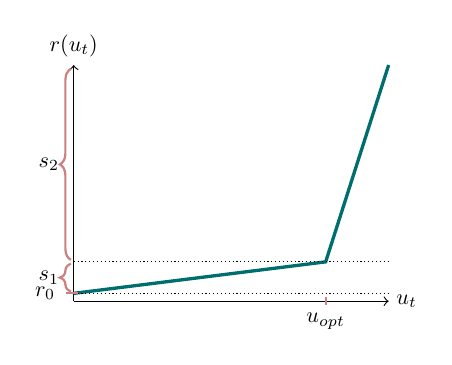
\begin{tikzpicture}[scale=0.5, every node/.style={scale=0.8}]
			
% Axis

\draw[->] (0,0) -- (0,6) node [above ]{$r(u_t)$};
\draw[->] (0,0) -- (8,0) node [right] {$u_t$};


% Slopes and lines

\draw [darkmint, very thick](0,0.2) -- (6.4,1) -- (8,6);

\draw [densely dotted, thin] (0,1) -- (8,1);
\draw [densely dotted, thin] (0,0.2) -- (8,0.2);

% Labels and Braces

\draw [thick, lightred] (6.4,0.1) -- (6.4,-0.1) node [below, align = center, text = black] {$u_{opt}$};

\draw [thick, lightred] (-0.2,0.2) -- (0.1,0.2) node [xshift = -6.5pt, left, align = right, text = black] {$r_0$};

%\draw [decorate,decoration={brace,amplitude=2pt},xshift=-2pt,yshift=0pt](0,0) -- (0.0,0.12) node [black,midway,xshift=-0.3cm] {$r_0$};

\draw [decorate,decoration={brace,amplitude=4pt},xshift=-2pt,yshift=0pt, lightred, thick](0,0.25) -- (0.0,0.95) node [black,midway,xshift=-0.35cm] {$s_1$};

\draw [decorate,decoration={brace,amplitude=4pt},xshift=-2pt,yshift=0pt, lightred, thick](0,1.05) -- (0,5.9) node [black,midway,xshift=-0.35cm] {$s_2$};
		\end{tikzpicture}
		\caption{Dual Interest Slope}
	\end{figure}
\end{minipage}
\begin{minipage}{0.38\textwidth}
	\vspace{-1em}
	\begin{equation*}
		u_t = \dfrac{D_t}{L_t}
	\end{equation*}
	
	\vspace{0.5 em}
	Two interest slopes set incentives for borrowing when utilization is below optimal $u_{opt}$ and repayment if its above, threatening the lenders' ability to withdraw assets.
	
\end{minipage}	
}

\end{frame}
%%%	


%%%
\begin{frame}{CDM: Borrower's Interest and Lender's Yield }

In a CDM applying two interest slopes for an asset defined by the tuple $(r_{min}, r_{opt}, r_{max}, u_{opt})$, current $r_b$ accrued by borrowers can be expressed as follows:


\begin{equation*}
	r_b = 
		\begin{cases}
		r_{min} + \dfrac{u_t}{u_{opt}}(r_{opt}-r_{min}), & \text{if } u_t \leq u_{opt} \vspace{1em}\\
		r_{opt} + \dfrac{u_t-u_{opt}}{1-u_{opt}}(r_{max}-r_{opt}), & \text{if } u_t > u_{opt}
		\end{cases}
\end{equation*}

\vspace{1em}

\uncover<2-> {
Accounting for a reserve factor $RF \in [0,1]$ deducted as income for the protocol, the $r_b$ collected from borrowers and attributed to the lenders of the asset as yield $r_l$ equals to:

\begin{equation*}
	r_l = u_t r_b (1-RF) 
\end{equation*}
}

\end{frame}
%%%	


%%%
\begin{frame}{A Borrower's Perspective}

With the transfer of collateral assets, \textbf{a credit line is opened }against which assets can be borrowed along the protocol’s terms.

\vspace{0.8 em}
Within CDMs, the collateral commonly becomes part of the assets available for borrowing, i.e., \textbf{a borrower is also a lender.}

\uncover<2-> {
\vspace{0.8 em}
A borrower must continuously \textbf{monitor prices} of collateral and debt assets incl. interest accrued, to avoid their \textbf{position becoming unhealthy}.

\vspace{0.8 em}
If liquidated, a position is \textbf{commonly subject to some penalty} funding the incentivation of liquidators.
}

\uncover<3-> {
\vspace{0.8 em}
\begin{keytakeaway}{Limited Risk for Borrowers}
	Risk of the borrower is effectively limited to the difference between collateral locked and debt drawn, as there is very limited effective recourse to compel repayment of borrowed assets. 
\end{keytakeaway}
}
	
\end{frame}
%%%	


%%%
\begin{frame}{Overcollateralization and Liquidation}

Protocols require a \textbf{minimum overcollateralization} in the pseudoanonymous DeFi environment, i.e., $d \leq c \cdot LT$.
\vspace{1em}

\begin{minipage}{0.6\textwidth}
	\vspace{1.5em}
	\begin{figure}[t]
		\centering
		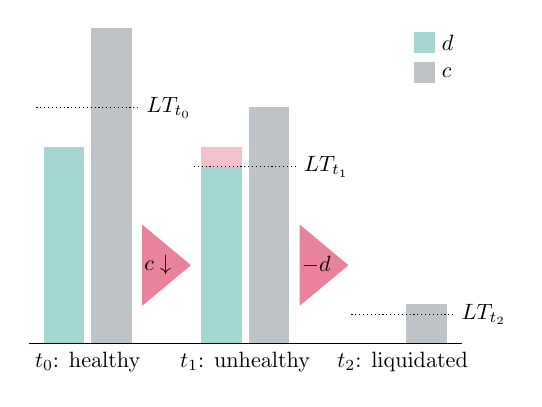
\begin{tikzpicture}[scale=0.5, every node/.style={scale=0.8}]
			
% t0

\filldraw[color = mint] (0.4,0) rectangle ++(1,5);
\filldraw[color = brightanthracite] (1.6,0) rectangle ++(1,8);

\draw [densely dotted, thin] (0.2,6) -- (2.8,6) node [right, text = black]{$LT_{t_0}$};

% t1
\uncover<2-> {
	\draw [softred, fill = softred] (2.9,3) -- (4.1,2) -- (2.9,1) -- (2.9,3) node [midway,right, text = black, xshift = -0.1cm] {$c \downarrow$} -- cycle;

	\filldraw[color = mint] (4.4,0) rectangle ++(1,5);
	\filldraw[softred!50] (4.4,4.5) rectangle ++(1,0.5);
	\filldraw[color = brightanthracite] (5.6,0) rectangle ++(1,6);

	\draw [densely dotted, thin] (4.2,4.5) -- (6.8,4.5) node [right, text = black]{$LT_{t_1}$};
}


% t2

\uncover<3->{
	\draw [softred, fill] (6.9,3) -- (8.1,2) -- (6.9,1) -- (6.9,3) node [midway,right, text = black, xshift = -0.1cm] {$-d$}  -- cycle;

	\filldraw[color = brightanthracite] (9.6,0) rectangle ++(1,1);


	\draw [densely dotted, thin] (8.2,0.75) -- (10.8,0.75) node [right, text = black]{$LT_{t_2}$};
}

% Axis with labels

\draw[-] (0,0) -- (1.5,0) node [below]{$t_0$: healthy} -- (5.5,0) node [below]{$t_1$: unhealthy} -- (9.5,0) node [below]{$t_2$: liquidated} -- (11,0);

\filldraw [mint] (9.8,7.4) rectangle ++ (0.5,0.5);
\node	at (10.3,7.65) [right] {$d$};

\filldraw [brightanthracite] (9.8,6.65) rectangle ++ (0.5,0.5);
\node	at (10.3,6.9) [right] {$c$};
		\end{tikzpicture}
		\caption{Scenario with $LT = 0.75$}
	\end{figure}
\end{minipage}
\begin{minipage}{0.38\textwidth}
	
	\uncover<2->{
	If collateral value relative to the debt falls below $LT$, the risk of borrower default is too high, i.e., the position state is \emph{unhealthy}.
	}
	
	\vspace{1em}
	\uncover<3->{
	Collateral can now be liquidated by anyone against repayment of the 		position’s debt.
	}
\end{minipage}
	
\end{frame}
%%%	


%%%
\begin{frame}{Liquidations: Two Approaches (cont.)}

With protocols unable to become active by themselves, they \textbf{rely on arbitrageurs} to spot and liquidate unhealthy positions.

\uncover<2->{
\vspace{1 em}
Two approaches offering liquidation incentives can be observed: 

\vspace{1 em}
\textbf{1. Discount Sale} (e.g. Aave or Compound)
\vspace{0.2em}
\begin{itemize}
\item Any unhealthy position’s collateral is offered at a discount from the current on-chain oracle price.
\item Liquidator repays (part of the) position’s debt in the respective debt asset and in return receives collateral assets at the discounted price for the repaid amount.
\end{itemize}

\vspace{0.5em}
\textbf{Pro:} Atomic transaction, fast.

\textbf{Con:} Requires high accuracy of on-chain oracle prices at all times.
}

\end{frame}
%%%	


%%%
\begin{frame}{Liquidations: Two Approaches }


\textbf{2. Collateral Auction}\\
\vspace{0.2em}
Collateral price discovery via auctions, avoiding fixed liquidator incentives. Example of a format employed by MakerDAO \cite{MakerDAO}:
\begin{itemize}
\item Dutch auction with starting price defined by oracle module. 
\item Collateral price decreases over time. 
\item Liquidators can buy any still available proportion of the collateral at current price.
\item Closes, when all debt is covered. Resets, if price falls below a certain ratio to the starting price or a duration limit is reached.
\end{itemize}
\vspace{0.5em}

\textbf{Pro:} Potentially leaving borrowers with a better collateral price.\\
\vspace{0.5em}
\textbf{Con:} Heavily depending on auction format. Considerations must be given to duration, lower-bound for  prices, oracle role, and resilience during network congestions driving cost of timely transactions.


	
\end{frame}
%%%	


%%%
\begin{frame}{Flash Loans Overview}

\begin{minipage}{0.3\textwidth}
	\begin{figure}
		\includegraphics[width=0.7\textwidth]{../assets/images/flashloan}	
	\end{figure}
\end{minipage}
\begin{minipage}{0.65\textwidth}
	Flash loans are a \textbf{concept unique to DeFi}. They are the only loans in the ecosystem that \textbf{do not require collateral}.
\end{minipage}

\vspace{2em}

\uncover<2-> {
\begin{minipage}{0.6\textwidth}

	Funds are borrowed, used, and repaid \textbf{all in one transaction}.

	\vspace{1em}
	Instead of collateral, lenders rely on \textbf{transaction atomicity}: If principal plus fee is not paid back, all is reverted as if the funds were never granted.
\end{minipage}
\begin{minipage}{0.38\textwidth}
	\begin{figure}
		\begin{tikzpicture}[scale=0.8, every node/.style={scale=0.8}]
			
% Burger

\node at (0,0) {\includegraphics[height = 4cm]{../assets/images/burger}};

% Labels

\node at (0, 1.1) [text = darkmint] {\textbf{Borrow funds}};

\node at (0,-0.1) [text = darkmint, fill = white!50] {\textbf{Use funds at discretion}};

\node at (0,-1.3) [text = darkmint] {\textbf{Repay funds + fees}};


% Arrows

\draw [softred, fill = softred] (-0.4,0.7) -- (0.4,0.7) -- (0,0.3) -- (-0.4,0.7)  -- cycle;

\draw [softred, fill = softred] (-0.4,-0.6) -- (0.4,0-0.6) -- (0,-1) -- (-0.4,-0.6)  -- cycle;



		\end{tikzpicture}	
	\end{figure}
\end{minipage}
}

\end{frame}
%%%	


%%%
\begin{frame}{Flash Loan Conditions}
For a successful flash loan of $x$ with interest $\rho$  and / or a flat fee $\varphi$:

\vspace{1em}
\begin{enumerate}
	\item The lending market must \textbf{have $x$ liquid available.}\\
	\begin{equation*}
		x \leq LP_{x}
	\end{equation*}
	(Unless borrowed from a CDP, where $x$ can be \textit{flash-minted})
	\vspace{1em}
	\item The whole principal plus all interest and fees ($ x(1+\rho) + \varphi$) must be \textbf{returned at the end of the transaction.}
\end{enumerate}

\uncover<2->{
\vspace{1em}

\begin{keytakeaway}{Failing Flash Loans}
	If conditions are not met, the flash loan transaction is still included in the blockchain but is considered failed, i.e., it does not lead to any state changes except for a nonce update and transaction fee $\epsilon$. 
\end{keytakeaway}
}

	
\end{frame}
%%%	


%%%
\begin{frame}{Example of Arbitrage with Flash Loan}

With $x$ as the amount borrowed and sold at the high-price exchange and $x^\ast$ the amount bought back at the low-price exchange with the proceeds, the payoff $\Pi$ can be expressed as:

\begin{equation*}
	\Pi = max (x^{\ast}-[x \,(1+\rho) + \varphi ],0) - \epsilon
\end{equation*}

\vspace{0.5 em}

\uncover<2->{
\begin{minipage}{0.60\textwidth}
	\begin{figure}[t]
		\centering
		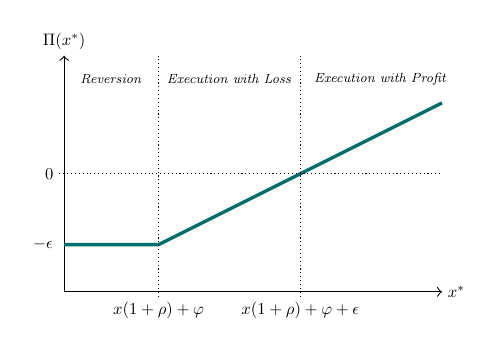
\begin{tikzpicture}[scale=0.6, every node/.style={scale=0.6}]
			
% Axis

\draw[->] (0,0) -- (0,5) node [above ]{$\Pi(x^\ast)$};
\draw[->] (0,0) -- (8,0) node [right] {$x^\ast$};


% Slope

\draw [darkmint, very thick](0,1) node [left, xshift = -0.1cm, black]{$-\epsilon$} -- (2,1) -- (8,4);


% Lines and Labels

\draw [densely dotted, thin] (-0.1,2.5)node [left, black] {$0$} -- (8,2.5);

\draw [densely dotted, thin] (2,-0.1) node [below, black]{$x(1 + \rho) + \varphi$} -- (2,5);

\draw [densely dotted, thin] (5,-0.1) node [below, black]{$x(1 + \rho) + \varphi + \epsilon$} -- (5,5);

\footnotesize

\node at (1,4.5) {\textit{Reversion}};

\node at (3.5,4.5) {\textit{Execution with Loss}};
\node at (6.7,4.5) {\textit{Execution with Profit}};
		\end{tikzpicture}
		\caption{Flash Loan Payoff Diagram \cite{FS21FlashLoans}}
	\end{figure}
\end{minipage}
\begin{minipage}{0.38 \textwidth}
\vspace{-1em}
	Is a corresponding flash loan available when a token pair has a significant price difference on-chain, \textbf{anyone can become an arbitrageur }with the loss potential capped at transaction fee $\epsilon$.
\end{minipage}
}
	
\end{frame}
%%%	


%%%
\begin{frame}{Consequence of Flash Loans}

Flash loans \textbf{effectively remove capital} constraints for any activity that can be performed in one transaction.

\vspace{1em}

\uncover<2->{
\textbf{Common Use Cases}:

\begin{itemize}
\item Collateral swaps (original use case).
\item Arbitrage.
\item Portfolio Refactoring.
\item Price Manipulation and Wash Trading.

\end{itemize}
}

\vspace{2em}

\uncover<3->{
$\Rightarrow$ While it arguably can be missused, the unique DeFi tool of flash loans have the potential to make markets more efficient and fair.
}

	
\end{frame}
%%%	


%%%
\begin{frame}%[allowframebreaks]

\frametitle{References and Recommended Reading}

	\bibliographystyle{amsplain}
	\bibliography{../assets/bib/refs}
\end{frame}
%%%



\end{document}